\documentclass[12pt,a4paper, red]{bbe}
\usepackage{blindtext}
\usepackage{listings}
\usepackage{xcolor}
\usepackage{subfiles}
\usepackage{hyperref} %for Hyperlinks

\definecolor{codegreen}{rgb}{0,0.6,0}
\definecolor{codegray}{rgb}{0.5,0.5,0.5}
\definecolor{codepurple}{rgb}{0.58,0,0.82}
\definecolor{codebackcolour}{rgb}{0.95,0.95,0.92}

  	
%added be me.
%Code listing style named "mystyle"
\lstdefinestyle{mystyle}{
    backgroundcolor=\color{codebackcolour},
    commentstyle=\color{codegreen},
    keywordstyle=\color{magenta},
    numberstyle=\tiny\color{codegray},
    stringstyle=\color{codepurple},
    basicstyle=\ttfamily\footnotesize,
    breakatwhitespace=false,         
    breaklines=true,                 
    captionpos=b,                    
    keepspaces=true,                 
    numbers=left,                    
    numbersep=5pt,                  
    showspaces=false,                
    showstringspaces=false,
    showtabs=false,                  
    tabsize=2
}

\lstset{style=mystyle}

\begin{document}
    \setcounter{chapter}{1}
	\chapter{Calculations}
	
	\section{Basic calculations }
	
	After you have created some variables we can now use them with different mathematical operators to perform calculations. Lets start with some basic arithmetic.
	
	\vspace{5mm}
	
	\begin{lstlisting}
    age = 17
    age = age + 1
    print(age)\end{lstlisting}
	
    After running this with the > button it should print 18
    
    \begin{lstlisting}
    > 18\end{lstlisting}
    
    \vspace{5mm}
    
    
    The identifier/variable 'age' will store the integer 17. In line 2 age will be increased by 1.
    In this example the number '1' is called a 'literal' - an actual value. Variables can be be added to variables.
    
    \begin{lstlisting}
    score = 100
    enemy_value = 5
    score = score + enemy_value
    print(score)\end{lstlisting}
    
    In this example the score will be increase by 5. And the output is shown below.
    
    \begin{lstlisting}
    > 105\end{lstlisting}
    
    The are different mathematical operations that can be performed:
    \begin{itemize}[c]
	    \item Addition  +
	    \item Subtraction -
	    \item Multiplication *
	    \item Division /
	    
	\end{itemize}
	
	\begin{remark}
	Have a go at at using the other operators.
	\end{remark}
	
	Some example cases:
	
	\begin{lstlisting}
    bill = 20.50
    VAT = 0.20
    VAT_to_pay = bill * VAT
    total = bill + VAT_to_pay
    print(total)\end{lstlisting}
    
    This will print out as shown below
    
    \begin{figure}[h]
        \centering
        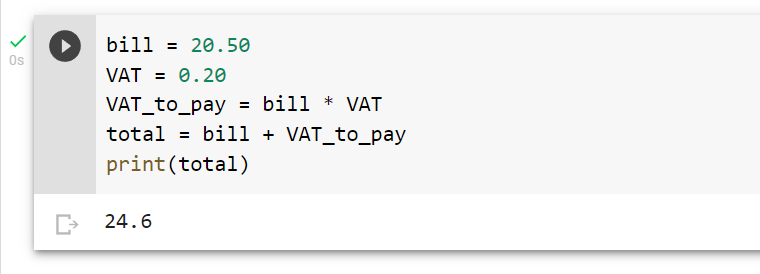
\includegraphics[width=0.5\textwidth]{images/ch2/bil.PNG}
        \caption{Output from google colab}
    \end{figure}
    
    The caluclations are correct, the answer is right, but python does not know this is money and does not show the formatting that we may expect. Further in the book we will fix this to make it output as below.
    
    \begin{lstlisting}
    > 24.60\end{lstlisting}
    
\section{Order of opperations}

	When performing operation the computer will use BIDMAS or BODMAS. It will take into account the order that opperations should be performed. For example look at the 2 line of code below.
\end{document}

\beging{listing}
a = 2 + 4 * 3
b = (2 + 4) * 3
print(a)
print(b)\end{listing}

The 2 calculations have the same operators but they are performed in a different order. Multiplication is performed before addition. If we want to add first we have to enclose the addition in brackets. This will output the following:

\begin{lstlisting}
    > 14
    > 18\end{lstlisting}
    
Its really important to consider this when using mathematical operations in your code.

\section{Modulo Operator}

In addition to the usual 4 operators the modulo operator is very useful in programming. It works by calculating the remainder after a number has been divided. A few examples will help to clarify this.
\begin{listing}
n = 5 % 2
print(n)\end{listing}

In this example 5 is divided by 2, the output is shown below:

\begin{listing}
> 1
\end{listing}

The answer is 1 as 5 / 2 is 2 with a remainder of 1. Modulo is the remainder part.
This is used in everyday life with clocks and the 12 hour clock. The code below shows how we could use modulo
to convert 24 hour time to 12 hour time.

\begin{listing}
time = 17 % 12
print(time)\end{listing}

The above code shows 17:00 in 12 hour clock would be:

\begin{lising}
> 5
\end{lising}

This is because 17 / 12 is 1 remainder 5.  One full 12 hours, and 5 more. A total of 17




